\documentclass[11pt]{scrartcl}

% =========================================================
% Page geometry + spacing
% =========================================================
\usepackage[a4paper,margin=1in]{geometry}
\usepackage{setspace}
\onehalfspacing
\usepackage[protrusion=false,expansion=false]{microtype}
\KOMAoptions{parskip=half, fontsize=11pt}

% =========================================================
% Math + tables + links
% =========================================================
\usepackage{amsmath,amssymb,amsfonts,amsthm}
\usepackage{booktabs}
\usepackage{longtable}
\usepackage{float}
\usepackage{caption}
\usepackage{enumitem}
\usepackage{array}

\usepackage{hyperref}
\hypersetup{
  colorlinks=true,
  linkcolor=blue,
  citecolor=blue,
  urlcolor=blue
}

% =========================================================
% Figures (TikZ/PGFPlots)
% =========================================================
\usepackage{tikz}
\usetikzlibrary{arrows.meta,positioning,calc}
\usepackage{pgfplots}
\pgfplotsset{compat=1.18}
\pgfplotsset{
  every axis/.append style={
    width=\textwidth,
    height=7.5cm,
    tick label style={font=\small},
    label style={font=\small},
    legend style={font=\small},
    title style={font=\small},
    grid=major
  }
}

% =========================================================
% Code listings
% =========================================================
\usepackage{listings}
\usepackage{xcolor}
\lstdefinestyle{py}{
  language=Python,
  basicstyle=\ttfamily\small,
  keywordstyle=\bfseries,
  commentstyle=\itshape\color{gray},
  stringstyle=\color{blue!60!black},
  showstringspaces=false,
  breaklines=true,
  frame=single,
  rulecolor=\color{black!20},
  tabsize=2
}

% =========================================================
% Theorem-like environments
% =========================================================
\newtheorem{definition}{Definition}[section]
\newtheorem{proposition}{Proposition}[section]
\newtheorem{remark}{Remark}[section]

% =========================================================
% Headers/Footers
% =========================================================
\usepackage{fancyhdr}
\pagestyle{fancy}
\fancyhf{}
\lhead{\small Limit Order Book Information and Tradable Alpha}
\rhead{\small \thepage}

% =========================================================
% Title
% =========================================================
\title{\textbf{When Does Limit Order Book Information Constitute Tradable Alpha?}\\[0.5em]
\large Explicit predictive gates, cost-aware evaluation, cross-sectional inference,\\and reproducibility}
\author{William Odumosu\\\normalsize Independent Researcher}
\date{August 2026}

\begin{document}
\maketitle

\begin{abstract}
Limit order book signals are commonly reported on the strength of a rank correlation and a cumulative profit curve. Such reports frequently leave three questions open: whether the effect holds on each instrument in a panel or on the most active alone, whether the significance withstands the number of hypotheses evaluated, and whether the predicted movement exceeds the spread that must be crossed to trade it. This paper sets out a protocol that separates the three. Using five NASDAQ instruments from the LOBSTER sample (AAPL, AMZN, GOOG, INTC, and MSFT; 953{,}829 clean events), I evaluate four microstructure signals against four sequential gates: cross-sectional predictive power, Benjamini--Hochberg correction at the full hypothesis budget of 1{,}080, positive gross profit, and profitability net of a parameterised cost model. Order flow imbalance, queue imbalance, and micro-price deviation clear the first three gates, with rank information coefficients between 0.10 and 0.19 holding the same sign on all five instruments. None clears the fourth. The strongest signal reaches breakeven at 4.8\% of the assumed half-spread, and costs account for 2{,}099\% of gross profit under the baseline assumption. Two further results follow from the panel structure: queue imbalance and micro-price deviation function as a single signal, with a rank correlation of 0.969 and an incremental out-of-sample $R^2$ of $-0.0006$; and order flow imbalance dominates on the wide-spread, thin-queue instruments while the top-of-book signals dominate on the penny-spread, deep-queue instruments, with the ordering reversing between the two groups. A Python implementation with 80 tests and synthetic controls of known ground truth accompanies the paper.
\end{abstract}

\vspace{0.5em}
\noindent\textbf{Keywords:} limit order book, market microstructure, order flow imbalance, queue imbalance, micro-price, transaction costs, high-frequency data, multiple testing, backtest overfitting, reproducibility

\noindent\textbf{JEL classification:} G14, G17, C58, C52, C12

\vspace{0.8em}
\noindent\textbf{AI disclosure.} This work was produced by the author working in tandem with Anthropic's Claude. The author framed the research programme, wrote the project outline specifying the signal set, horizons, validation strategy, cost treatment, and robustness battery, and directed the sequence in which the work was carried out. The model was used to implement the accompanying Python framework against that specification, to run the analysis pipeline, and to produce initial drafts of this manuscript. The author acquired the data, edited the codebase, reviewed and revised the text, and verified the reported figures against the pipeline's output tables. Several methodological errors surfaced during that review process and are documented in Remarks~\ref{rem:pooling} and~\ref{rem:nulltrap} rather than quietly corrected.

\noindent\textbf{Data availability.} The LOBSTER academic samples used here are free downloads from \url{https://lobsterdata.com/info/DataSamples.php} and are not redistributed. The analysis code, configuration files, and all result tables are available at \url{https://github.com/study-holic/q1-lob-alpha} under an MIT licence.

\noindent\textbf{Declaration of interest.} None.

\newpage
\tableofcontents
\listoffigures
\listoftables
\newpage

% =========================================================
\section{Introduction}
\label{sec:intro}

Limit order book data permits unusually direct measurement of short-horizon predictability. The book state at time $t$ is observable, the mid-price at $t+h$ is observable, and the correlation between them is a well-defined quantity requiring no asset pricing model to interpret. The same conditions that make measurement easy also make several biases difficult to detect, since each arises from the structure of the data and not from an error in the analysis.

Four such biases operate on this dataset. A 100-event horizon evaluated at every event reuses each price move a hundred times, so overlapping forward returns inflate apparent significance. Serially correlated signals violate the independence assumption behind ordinary standard errors, and the resulting bias is upward. Pooling instruments into a single correlation yields an average weighted by event count, which on the panel used here means that two of five instruments contribute 80\% of the observations. Four signals evaluated across six horizons, nine regime cells, and five instruments constitute 1{,}080 hypotheses, of which 54 are expected to reach the five per cent level under a global null.

The word ``predictive'' is applied to four claims of increasing strength:

\begin{enumerate}[label=(\arabic*)]
\item A signal correlates with future returns.
\item A signal predicts future returns on every instrument in the panel.
\item A predictive signal generates positive gross profit.
\item A profitable signal remains profitable after execution costs.
\end{enumerate}

Each claim implies the one before it, and each requires evidence beyond what the previous claim requires. This paper evaluates four standard microstructure signals against all four claims on NASDAQ order book data, reporting the outcome of each stage separately for each signal.

\paragraph{Central question.} How much incremental information about short-horizon price movements is contained in limit order book state, and how much of that information remains after realistic execution costs?

On the data examined here, the answer to the first part is a great deal, and to the second, none. Rank information coefficients between 0.10 and 0.19 hold the same sign on all five instruments and clear Benjamini--Hochberg correction across the full hypothesis budget. The strongest signal reaches breakeven at 4.8\% of the assumed half-spread. The measured information is roughly twenty times smaller than the cost of acting on it, and Section~\ref{sec:failure} identifies the execution assumption as the single point at which it is lost.

\subsection{Contributions}
\label{sec:contributions}

\begin{enumerate}[label=(\arabic*)]
\item A four-gate protocol separating statistical significance, cross-sectional generality, gross profitability, and profitability net of costs, with each gate reported for every signal separately.
\item Rank information coefficients for four signals across six horizons on five instruments, with block bootstrap intervals, exact circular-shift $p$-values, and Benjamini--Hochberg correction at the full hypothesis budget of 1{,}080.
\item Evidence that order flow imbalance and the top-of-book signals capture different information and dominate at opposite ends of the liquidity spectrum.
\item A demonstration that queue imbalance and micro-price deviation constitute a single signal, established through rank correlation, variance inflation, and incremental out-of-sample $R^2$.
\item A cost sensitivity analysis locating the point at which a statistically significant signal ceases to be economically useful.
\item A reproducible implementation with synthetic controls of known ground truth, permitting a null result to be distinguished from a defective pipeline.
\end{enumerate}

% =========================================================
\section{Related work}
\label{sec:related}

Each of the three directional signals evaluated here has an established literature.

Order flow imbalance in the form used below is due to Cont, Kukanov, and Stoikov \cite{Cont2014}, who show that a change in displayed size is uninformative unless conditioned on whether the price level moved. Queue imbalance appears throughout the microstructure literature as a proxy for short-term directional pressure, without a single canonical formulation. The micro-price is due to Stoikov \cite{Stoikov2018}, who derives it as an estimate of fair value between the quotes under unbalanced queues.

The methodological literature bears directly on the design used here. Harvey, Liu, and Zhu \cite{Harvey2016} and Bailey and L\'opez de Prado \cite{Bailey2014} establish that the effective number of trials in empirical finance substantially exceeds the number reported, and that conventional significance thresholds are correspondingly uninformative. Both address cross-sectional asset pricing, where the researcher selects each specification deliberately. At event frequency the hypothesis count is instead generated mechanically by the choice of horizons and regime partitions, which raises the effective trial count without any corresponding decision by the researcher.

The signals evaluated here are therefore taken as given. What this paper tests is whether their conventional reporting withstands an explicit accounting of transaction costs, hypothesis count, and cross-sectional generality. Figure~\ref{fig:gates} sets out the protocol.

\begin{figure}[H]
\centering
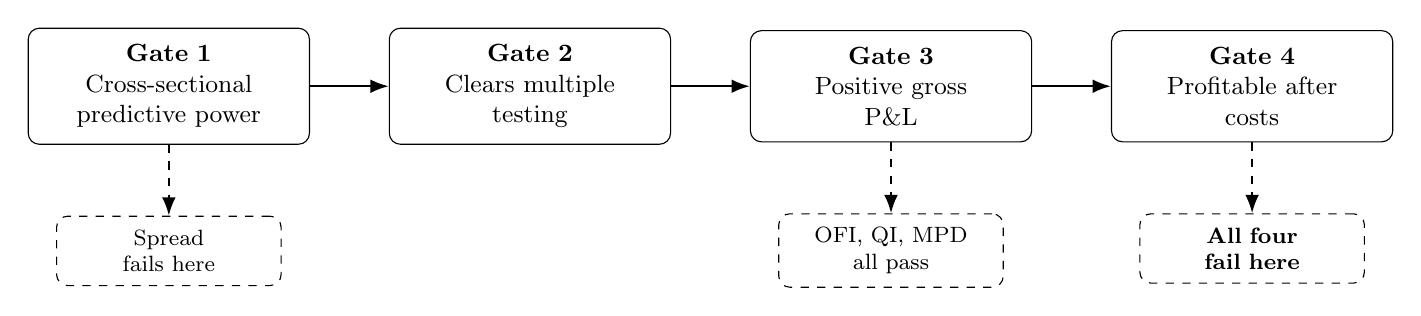
\begin{tikzpicture}[
  node distance=9mm and 10mm,
  box/.style={draw, rounded corners, align=center, inner sep=6pt, text width=3.15cm, font=\small},
  fail/.style={draw, dashed, rounded corners, align=center, inner sep=5pt, text width=2.5cm, font=\footnotesize},
  arr/.style={-Latex, thick}
]
\node[box] (g1) {\textbf{Gate 1}\\Cross-sectional\\predictive power};
\node[box, right=of g1] (g2) {\textbf{Gate 2}\\Clears multiple\\testing};
\node[box, right=of g2] (g3) {\textbf{Gate 3}\\Positive gross\\P\&L};
\node[box, right=of g3] (g4) {\textbf{Gate 4}\\Profitable after\\costs};

\node[fail, below=of g1] (f1) {Spread\\fails here};
\node[fail, below=of g3] (f3) {OFI, QI, MPD\\all pass};
\node[fail, below=of g4] (f4) {\textbf{All four}\\\textbf{fail here}};

\draw[arr] (g1) -- (g2);
\draw[arr] (g2) -- (g3);
\draw[arr] (g3) -- (g4);
\draw[arr, dashed] (g1) -- (f1);
\draw[arr, dashed] (g3) -- (f3);
\draw[arr, dashed] (g4) -- (f4);
\end{tikzpicture}
\caption{The four-gate protocol. Each gate states a stronger claim than the one before it, and a tradable signal must clear all four. On the data studied here, nothing reaches the far right.}
\label{fig:gates}
\end{figure}

% =========================================================
\section{Data}
\label{sec:data}

\subsection{Source and coverage}
\label{sec:source}

I use the free LOBSTER academic samples \cite{Huang2011}: full limit order book reconstructions from NASDAQ Historical TotalView-ITCH for five instruments on 21 June 2012, 09:30 to 16:00. Each instrument ships as two headerless CSVs, a message file and an orderbook file, with one row in each per book update. I use level~1 of the 10-level export.

The sample dates from 2012 and remains the standard public benchmark for this class of work \cite{Kercheval2015}. The methodology below applies unchanged to newer or larger data.

\begin{table}[H]
\centering
\caption{Coverage and characteristics after cleaning.}
\label{tab:coverage}
\begin{tabular}{lrrrrl}
\toprule
Instrument & Events & Median spread & Rel.\ spread (bps) & Median depth & Price range \\
\midrule
AAPL & 99{,}799  & \$0.15 & 2.58 & 208    & 577.48--588.19 \\
AMZN & 51{,}701  & \$0.13 & 5.87 & 232    & 220.52--226.03 \\
GOOG & 42{,}603  & \$0.29 & 5.13 & 208    & 563.73--579.82 \\
INTC & 374{,}864 & \$0.01 & 3.73 & 28{,}278 & 26.62--27.60 \\
MSFT & 384{,}862 & \$0.01 & 3.31 & 28{,}216 & 30.07--31.14 \\
\bottomrule
\end{tabular}
\end{table}

The five instruments fall into two groups on price, spread, and depth. AAPL, AMZN, and GOOG trade above \$220 with spreads of 13 to 29 cents and roughly 200 shares at the touch. INTC and MSFT trade near \$30 with one-cent spreads and queues over a hundred times deeper. Section~\ref{sec:predictive} shows that the signal results follow this division.

\subsection{Canonical representation}
\label{sec:canonical}

The pipeline operates on a single schema:
\begin{center}
\texttt{timestamp, instrument, bid\_price, bid\_size, ask\_price, ask\_size}
\end{center}
with optional deeper levels as \texttt{bid\_price\_2}, \texttt{bid\_size\_2}, and so on. Four invariants are asserted at load time: no crossed books, no locked books, strictly positive prices and sizes, and monotonic timestamps within each instrument-session.

Two features of the LOBSTER format require explicit handling. Prices are integers in units of one ten-thousandth of a dollar, so a raw value of 2239500 denotes \$223.95. Omitting the divisor rescales every relative spread by four orders of magnitude and leaves every rank correlation unchanged, so an IC-based check will not detect it. LOBSTER also pads empty book sides with sentinel prices of $\pm 9999999999$. These pass a positivity test on the ask side and yield a mid-price near half a million dollars.

\subsection{Sessions}
\label{sec:sessions}

An instrument's record is a sequence of trading sessions separated by gaps during which the price moves with no observed event, and is often handled as though it were one contiguous series. Every backward or forward looking operation in the pipeline groups by instrument \emph{and} session:

\begin{itemize}
\item Forward returns are missing at a session tail, so an overnight move is never labelled an $h$-event horizon.
\item Order flow accumulation, rolling $z$-scores, and regime labels reset at each session start.
\item Positions begin flat each session and earn nothing across the gap.
\end{itemize}

Sessions are assigned by calendar day for exchange-traded data, or by a gap threshold for continuous venues.

\begin{remark}[Detecting the failure]
Single-session data cannot distinguish this implementation from one that ignores session boundaries, since every guarding test passes under both. The defect first appears on multi-day data, at which point the affected results have already been produced. The synthetic controls in Appendix~\ref{sec:controls} therefore generate multi-session panels with an overnight gap by default, although the real data used here covers one day.
\end{remark}

\subsection{Cleaning}
\label{sec:cleaning}

Ten cleaning rules apply in a fixed order. Each removes rows for one stated reason and records the count, giving the audit in Table~\ref{tab:cleaning}.

\begin{table}[H]
\centering
\caption{Cleaning audit, 2{,}110{,}860 raw events. Retained: 953{,}829.}
\label{tab:cleaning}
\begin{tabular}{lrr}
\toprule
Rule & Rows dropped & Share \\
\midrule
Null level-1 field            & 0 & 0.00\% \\
Non-positive price            & 0 & 0.00\% \\
Non-positive size             & 0 & 0.00\% \\
Crossed book                  & 0 & 0.00\% \\
Locked book                   & 0 & 0.00\% \\
Trading halt (message type 7) & 0 & 0.00\% \\
Duplicate timestamp           & 156{,}171 & 7.40\% \\
Implausible price jump        & 0 & 0.00\% \\
Stale repeated quote          & 1{,}000{,}860 & 47.41\% \\
Session shorter than horizon  & 0 & 0.00\% \\
\bottomrule
\end{tabular}
\end{table}

The export writes a row for every book update at any depth, including updates that leave the touch unchanged, so 47\% of LOBSTER rows are byte-identical to their predecessor at level~1. Each such row contributes a forward return of exactly zero to the target and an order flow increment of exactly zero to the signal. Retaining them inflates the sample, deflates measured volatility, and attenuates every correlation by a factor set by the instrument's depth activity.

That factor varies across the panel. Stale level-1 rows account for 32.8\% of observations on INTC and 37.1\% on MSFT, against 69.4\% on GOOG, 74.0\% on AAPL, and 80.2\% on AMZN. Retaining them would attenuate measured ICs unevenly by instrument, and Section~\ref{sec:where} treats cross-instrument differences of that kind as a result. The penny-spread names update their touch more frequently, since a one-cent grid places most size changes at the best quote.

% =========================================================
\section{Market microstructure signals}
\label{sec:signals}

The signal set was fixed at four before any result was computed.

\subsection{Order flow imbalance}
\label{sec:ofi}

The change in bid size minus the change in ask size conflates three events: a queue growing through arrivals, a queue shrinking through cancellations, and a queue disappearing when the price level moves. Conditioning on the price move distinguishes them.

For consecutive book states $n-1$ and $n$, the bid side contribution is
\begin{equation}
e^b_n = \mathbb{1}\{P^b_n \geq P^b_{n-1}\}\, Q^b_n \; - \; \mathbb{1}\{P^b_n \leq P^b_{n-1}\}\, Q^b_{n-1},
\label{eq:ofibid}
\end{equation}
which reads as three cases:

\begin{itemize}
\item \textbf{Bid price up}: the entire new queue is fresh demand, contributing $+Q^b_n$.
\item \textbf{Bid price unchanged}: the change in queue size gives the contribution, $Q^b_n - Q^b_{n-1}$.
\item \textbf{Bid price down}: the old queue was consumed or pulled, contributing $-Q^b_{n-1}$.
\end{itemize}

The ask side mirrors this with the inequalities reversed, and
\begin{equation}
\mathrm{OFI}_n = e^b_n - e^a_n,
\label{eq:ofi}
\end{equation}
so buying pressure is positive by construction. The per-event increment is noisy, and the reported signal is a rolling sum over a 20-event window, normalised by trailing mean depth over 200 events. The normalisation makes the signal comparable across instruments and across time within an instrument.

The normalisation is required on this panel. INTC's queues are over a hundred times deeper than GOOG's, and an unnormalised OFI would order the two names by depth.

Unit tests verify each branch of the definition against a hand-constructed two-row book, together with a side-reflection antisymmetry check.

\subsection{Queue imbalance}
\label{sec:qi}

\begin{equation}
QI_t = \frac{Q^b_t - Q^a_t}{Q^b_t + Q^a_t}, \qquad QI_t \in [-1, 1].
\label{eq:qi}
\end{equation}

Whether positive queue imbalance precedes a price rise is treated as an empirical question. Section~\ref{sec:predictive} finds that it does, on all five instruments.

\subsection{Micro-price deviation}
\label{sec:mpd}

\begin{align}
\mathrm{MicroPrice}_t &= \frac{P^a_t Q^b_t + P^b_t Q^a_t}{Q^b_t + Q^a_t}, \label{eq:micro}\\[4pt]
MPD_t &= \frac{\mathrm{MicroPrice}_t - m_t}{m_t}. \label{eq:mpd}
\end{align}

The ask price carries the \emph{bid} size as its weight, so a large bid queue moves the estimate towards the ask. The level is non-stationary and dominated by the price itself, and the analysis uses the deviation from the mid.

\begin{remark}[Algebraic near-equivalence]
\label{rem:algebra}
Micro-price deviation and queue imbalance are related by $MPD_t = \frac{s_t}{2 m_t}\, QI_t$, a scaling by half the relative spread. Section~\ref{sec:redundancy} measures the empirical consequence, which is that the two behave as one signal.
\end{remark}

\subsection{Spread}
\label{sec:spread}

\begin{equation}
s_t = P^a_t - P^b_t, \qquad \text{relative spread} = s_t / m_t.
\label{eq:spread}
\end{equation}

The spread enters the signal set as a candidate directional predictor and as a conditioning variable for the regime analysis. Sections~\ref{sec:predictive} and~\ref{sec:regimes} evaluate both roles.

% =========================================================
\section{Experimental methodology}
\label{sec:method}

\subsection{Targets}
\label{sec:targets}

Forward mid returns
\begin{equation}
r_{t,h} = \frac{m_{t+h} - m_t}{m_t}
\label{eq:fwd}
\end{equation}
are computed over horizons of 1, 5, 10, 25, 50, and 100 events. Event frequency differs by two orders of magnitude across this panel, so every horizon is also reported in elapsed seconds.

\begin{table}[H]
\centering
\caption{Event horizons in clock time, pooled.}
\label{tab:clock}
\begin{tabular}{rrrr}
\toprule
Horizon (events) & Median (s) & Mean (s) & 95th pct.\ (s) \\
\midrule
1   & 0.0001 & 0.12  & 0.64 \\
5   & 0.004  & 0.61  & 3.25 \\
10  & 0.024  & 1.23  & 6.10 \\
25  & 0.359  & 3.07  & 14.07 \\
50  & 1.450  & 6.13  & 26.91 \\
100 & 4.418  & 12.27 & 51.74 \\
\bottomrule
\end{tabular}
\end{table}

Event arrival is clustered, and a 100-event horizon spans a median of 4.4 seconds against a mean of 12.3 seconds. A decay result stated in events alone therefore admits two clock-time readings differing by a factor of three.

\subsection{Headline metric}
\label{sec:metric}

The headline metric is rank IC, the Spearman correlation between the signal at time $t$ and the forward return over the next $h$ events. Rank IC is invariant to monotone rescaling of the signal, and its reliance on ranks limits the influence of the fat tails present in high-frequency returns.

\subsection{Inference under time dependence}
\label{sec:inference}

Overlapping forward returns and autocorrelated signals violate the independence assumption behind ordinary standard errors, and the resulting bias is upward. Two procedures are used throughout:

\begin{itemize}
\item \textbf{Circular block bootstrap} for confidence intervals, block length 2{,}000 events, preserving local dependence within each resampled block.
\item \textbf{Circular-shift permutation} for $p$-values, shifting the signal so each series keeps its own autocorrelation while the alignment between them is destroyed. That is the correct null: ``this looks predictive purely because both series are persistent.'' The test is evaluated \emph{exactly}: a single cross-correlation gives the statistic at all $n$ shifts at once, and the null is enumerated over every admissible shift, roughly 950{,}000 on this panel. The procedure has no sampling floor, requires no seed, and runs in under a second.
\end{itemize}

\subsection{Cross-sectional aggregation}
\label{sec:crosssec}

A single Spearman correlation over the pooled panel is an average weighted by event count, and gives no indication of whether one instrument accounts for the whole effect. MSFT and INTC contribute 80\% of the rows here.

Rank IC is reported both pooled and per instrument, with a standard error taken across instruments:
\begin{equation}
t_{\mathrm{cross}} = \frac{\overline{IC}}{\hat{\sigma}_{IC} / \sqrt{N}},
\label{eq:tcross}
\end{equation}
where $N$ is the number of instruments. The statistic measures the generality of a signal across the panel, and is insensitive to its magnitude. A signal passes the predictive gate when $|t_{\mathrm{cross}}| > 3$ and the sign holds on every instrument.

\subsection{Validation geometry}
\label{sec:validation}

Splits are expanding-window and chronological, with a purge gap of 101 events. The gap exceeds the longest horizon by one, so no forward return terminates on a boundary. Threshold and signal selection occur on the validation slice, and the test slice is evaluated once per fold with no influence on any choice.

Splits are taken \emph{within each instrument}. The panel is stored instrument-major, so equal row blocks over the concatenated frame would assign one ticker's full trading day to a fold's test set and a different ticker's to its training set. Under that construction the purge gap falls between two unrelated stocks, and the holdout measures generalisation across names in place of generalisation across time. Every fold here contains all five instruments in each of its train, validation, and test blocks, as shown in Figure~\ref{fig:walkforward}.

\begin{figure}[H]
\centering
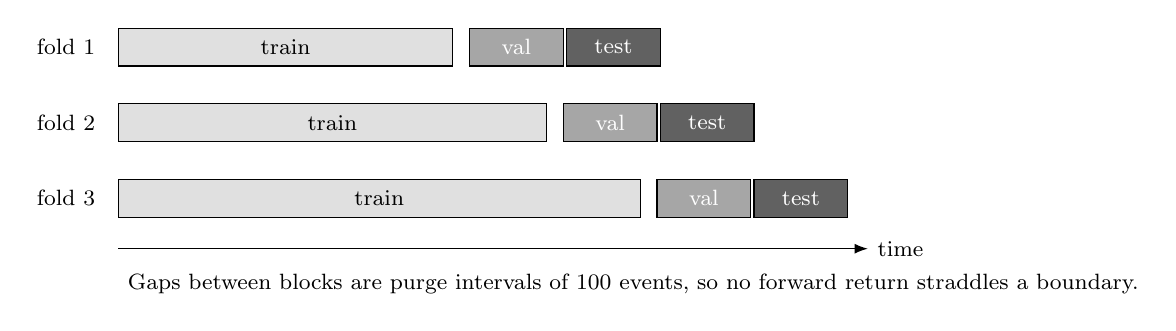
\begin{tikzpicture}[x=0.85cm, y=0.8cm, font=\small,
  trainbox/.style={draw, fill=black!12},
  valbox/.style={draw, fill=black!35},
  testbox/.style={draw, fill=black!62}]

% fold 1
\node[anchor=east, font=\footnotesize] at (-0.2,0.3) {fold 1};
\draw[trainbox] (0,0) rectangle (5.0,0.6);
\node[font=\footnotesize] at (2.5,0.3) {train};
\draw[valbox] (5.25,0) rectangle (6.65,0.6);
\node[font=\footnotesize, text=white] at (5.95,0.3) {val};
\draw[testbox] (6.7,0) rectangle (8.1,0.6);
\node[font=\footnotesize, text=white] at (7.4,0.3) {test};

% fold 2
\node[anchor=east, font=\footnotesize] at (-0.2,-0.9) {fold 2};
\draw[trainbox] (0,-1.2) rectangle (6.4,-0.6);
\node[font=\footnotesize] at (3.2,-0.9) {train};
\draw[valbox] (6.65,-1.2) rectangle (8.05,-0.6);
\node[font=\footnotesize, text=white] at (7.35,-0.9) {val};
\draw[testbox] (8.1,-1.2) rectangle (9.5,-0.6);
\node[font=\footnotesize, text=white] at (8.8,-0.9) {test};

% fold 3
\node[anchor=east, font=\footnotesize] at (-0.2,-2.1) {fold 3};
\draw[trainbox] (0,-2.4) rectangle (7.8,-1.8);
\node[font=\footnotesize] at (3.9,-2.1) {train};
\draw[valbox] (8.05,-2.4) rectangle (9.45,-1.8);
\node[font=\footnotesize, text=white] at (8.75,-2.1) {val};
\draw[testbox] (9.5,-2.4) rectangle (10.9,-1.8);
\node[font=\footnotesize, text=white] at (10.2,-2.1) {test};

\draw[-Latex] (0,-2.9) -- (11.2,-2.9) node[right, font=\footnotesize] {time};
\node[align=left, font=\footnotesize, anchor=north west] at (0,-3.15)
{Gaps between blocks are purge intervals of 100 events, so no forward return straddles a boundary.};
\end{tikzpicture}
\caption{Expanding-window validation geometry. Selection happens on the validation block; the test block is evaluated once per fold and never influences a choice.}
\label{fig:walkforward}
\end{figure}

\subsection{Look-ahead prevention}
\label{sec:lookahead}

Latency is enforced by the execution model, which applies a decision made at time $t$ to the book at $t+1$ at the earliest. The strategy interface exposes no path by which a signal can reach an earlier book state, so look-ahead is prevented by construction and not by convention. Z-scores and regime labels are computed from trailing windows. One test truncates the future of the sample and asserts that every past position is unchanged.

\subsection{Hypothesis budget}
\label{sec:budget}

Four signals, six horizons, nine regime cells, and five instruments give \textbf{1{,}080 hypotheses}, of which \textbf{54} are expected to appear significant at the five per cent level under a global null. Benjamini--Hochberg correction \cite{Benjamini1995} is applied at family size $m = 1{,}080$. The pooled table contains 24 rows, and a correction taken over those rows alone would account for a fraction of the specifications actually evaluated.

The family size determines what resolution the $p$-values require. The shift test evaluates every admissible circular shift of the signal by cross-correlation, giving a resolution near $10^{-6}$ on this panel. A sampled test at 300 draws has a floor of $0.0033$, which exceeds the rank-24 Benjamini--Hochberg threshold of $0.0011$ at $m = 1{,}080$, and would reject no hypothesis at that family size for any data.

\begin{remark}[Family size and the reported table]
\label{rem:family}
The $p$-values in Table~\ref{tab:pooled} are computed on the pooled table. The regime and per-instrument cells in Sections~\ref{sec:regimes} and~\ref{sec:where} were also evaluated, and any of them could have been selected for the headline. The relevant family comprises every hypothesis available for reporting, which is the count used here.
\end{remark}
% =========================================================
\section{Predictive results}
\label{sec:predictive}

\begin{table}[H]
\centering
\caption{Pooled rank IC by signal and horizon.}
\label{tab:pooled}
\begin{tabular}{lrrrrrr}
\toprule
Signal & $h{=}1$ & $h{=}5$ & $h{=}10$ & $h{=}25$ & $h{=}50$ & $h{=}100$ \\
\midrule
OFI                   & 0.083 & 0.132 & 0.150 & 0.150 & 0.158 & 0.168 \\
Queue imbalance       & 0.088 & 0.123 & 0.156 & 0.220 & 0.267 & 0.292 \\
Micro-price deviation & 0.074 & 0.115 & 0.150 & 0.219 & 0.274 & 0.306 \\
Spread                & 0.000 & 0.003 & 0.004 & $-0.000$ & $-0.001$ & 0.009 \\
\bottomrule
\end{tabular}
\end{table}

All eighteen cells for the first three signals survive Benjamini--Hochberg at $m = 1{,}080$; not one of the six spread cells does, with $p$-values from $0.39$ to $0.97$. Read alone, Table~\ref{tab:pooled} says that queue imbalance and micro-price deviation strengthen monotonically with horizon and reach a rank IC above 0.29.

Table~\ref{tab:cross} says something different.

\begin{table}[H]
\centering
\caption{Cross-sectional rank IC. Mean across the five instruments, with standard error and $t$-statistic. Bold rows mark each signal's strongest evidence. All six horizons are shown for the two top-of-book signals, so that the $|t| = 3$ gate crossing between $h=10$ and $h=25$ is visible rather than inferred; OFI and spread show a five-row and two-row selection respectively, and the full table is in \texttt{ic\_cross\_sectional.csv}.}
\label{tab:cross}
\begin{tabular}{lrrrrcrr}
\toprule
Signal & $h$ & Mean IC & SE & $t$ & Same sign & Min & Max \\
\midrule
OFI & 1   & 0.086 & 0.016 & 5.24 & 5/5 & 0.046 & 0.122 \\
OFI & 10  & 0.162 & 0.022 & 7.33 & 5/5 & 0.108 & 0.222 \\
\textbf{OFI} & \textbf{25} & \textbf{0.164} & \textbf{0.009} & \textbf{17.99} & \textbf{5/5} & 0.139 & 0.192 \\
OFI & 50  & 0.156 & 0.014 & 11.14 & 5/5 & 0.117 & 0.199 \\
OFI & 100 & 0.146 & 0.032 & 4.55 & 5/5 & 0.091 & 0.243 \\
\midrule
Queue imbalance & 1 & 0.114 & 0.017 & 6.87 & 5/5 & 0.083 & 0.178 \\
\textbf{Queue imbalance} & \textbf{5} & \textbf{0.150} & \textbf{0.021} & \textbf{7.32} & \textbf{5/5} & 0.081 & 0.198 \\
Queue imbalance & 10  & 0.163 & 0.037 & 4.46 & 5/5 & 0.063 & 0.263 \\
Queue imbalance & 25  & 0.182 & 0.065 & 2.80 & 5/5 & 0.034 & 0.357 \\
Queue imbalance & 50  & 0.189 & 0.085 & 2.22 & 5/5 & 0.018 & 0.410 \\
Queue imbalance & 100 & 0.183 & 0.099 & 1.86 & 5/5 & 0.011 & 0.426 \\
\midrule
\textbf{Micro-price dev.} & \textbf{1} & \textbf{0.105} & \textbf{0.014} & \textbf{7.56} & \textbf{5/5} & 0.081 & 0.159 \\
Micro-price dev. & 5   & 0.142 & 0.021 & 6.64 & 5/5 & 0.070 & 0.195 \\
Micro-price dev. & 10  & 0.156 & 0.037 & 4.24 & 5/5 & 0.054 & 0.257 \\
Micro-price dev. & 25  & 0.177 & 0.064 & 2.76 & 5/5 & 0.027 & 0.350 \\
Micro-price dev. & 50  & 0.189 & 0.086 & 2.20 & 5/5 & 0.014 & 0.414 \\
Micro-price dev. & 100 & 0.187 & 0.101 & 1.86 & 5/5 & 0.010 & 0.436 \\
\midrule
Spread & 1   & 0.005 & 0.005 & 1.07 & 3/5 & $-0.004$ & 0.022 \\
Spread & 100 & 0.006 & 0.012 & 0.49 & 4/5 & $-0.040$ & 0.034 \\
\bottomrule
\end{tabular}
\end{table}

Figure~\ref{fig:decay} plots both views. The pooled IC of queue imbalance rises from 0.088 to 0.292 as the horizon lengthens. Its cross-sectional $t$-statistic falls from 6.87 to 1.86 over the same range. Both are correct. The mean IC does rise, and the dispersion across instruments rises faster: at $h=100$ the per-instrument values span 0.011 to 0.426, a spread of nearly forty times.

\begin{figure}[H]
\centering
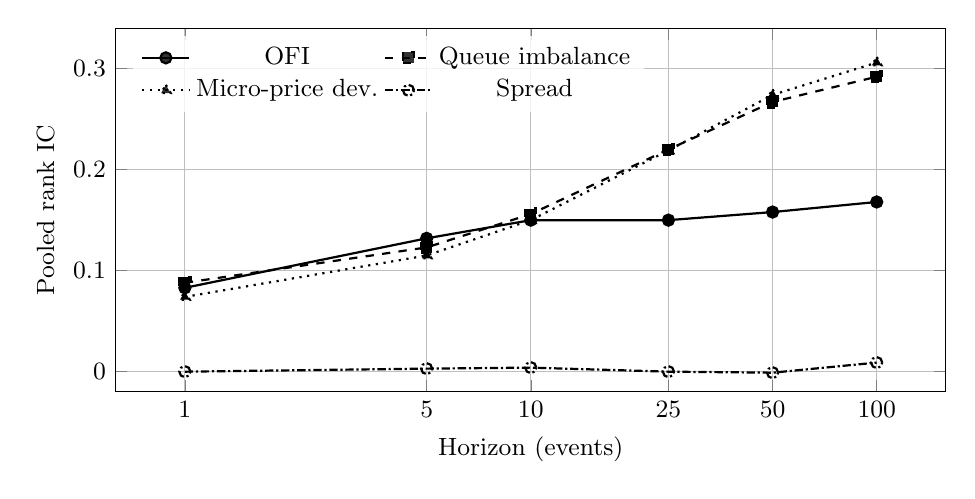
\begin{tikzpicture}
\begin{axis}[
  height=6.2cm,
  xlabel={Horizon (events)},
  ylabel={Pooled rank IC},
  xmode=log, log basis x=10,
  xtick={1,5,10,25,50,100}, xticklabels={1,5,10,25,50,100},
  legend columns=2,
  legend style={at={(0.02,0.98)},anchor=north west,draw=none,fill=white,fill opacity=0.8,text opacity=1},
  ymin=-0.02, ymax=0.34,
]
\addplot[mark=*,thick] coordinates {(1,0.083)(5,0.132)(10,0.150)(25,0.150)(50,0.158)(100,0.168)};
\addlegendentry{OFI}
\addplot[mark=square*,thick,dashed] coordinates {(1,0.088)(5,0.123)(10,0.156)(25,0.220)(50,0.267)(100,0.292)};
\addlegendentry{Queue imbalance}
\addplot[mark=triangle*,thick,dotted] coordinates {(1,0.074)(5,0.115)(10,0.150)(25,0.219)(50,0.274)(100,0.306)};
\addlegendentry{Micro-price dev.}
\addplot[mark=o,thick,densely dashdotted] coordinates {(1,0.000)(5,0.003)(10,0.004)(25,-0.000)(50,-0.001)(100,0.009)};
\addlegendentry{Spread}
\end{axis}
\end{tikzpicture}

\vspace{0.6em}

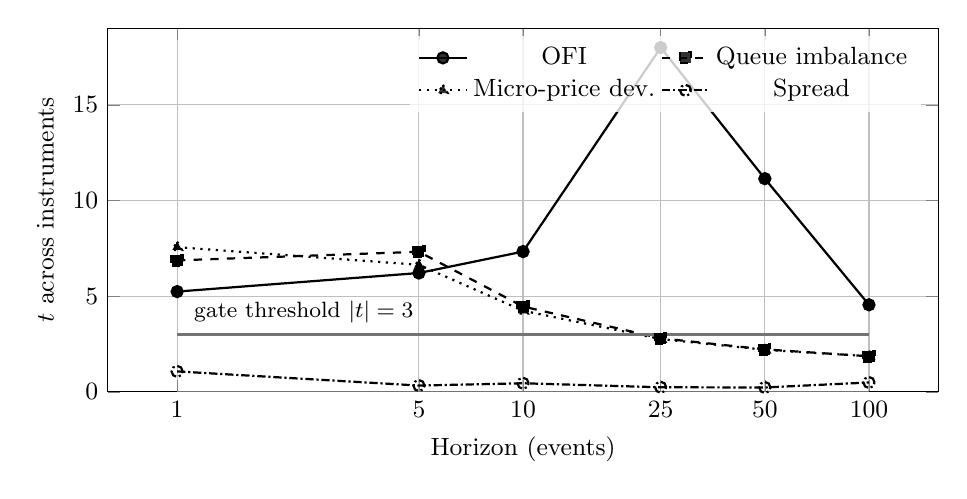
\begin{tikzpicture}
\begin{axis}[
  height=6.2cm,
  xlabel={Horizon (events)},
  ylabel={$t$ across instruments},
  xmode=log, log basis x=10,
  xtick={1,5,10,25,50,100}, xticklabels={1,5,10,25,50,100},
  legend columns=2,
  legend style={at={(0.98,0.98)},anchor=north east,draw=none,fill=white,fill opacity=0.8,text opacity=1},
  ymin=0, ymax=19,
]
\addplot[mark=*,thick] coordinates {(1,5.24)(5,6.21)(10,7.33)(25,17.99)(50,11.14)(100,4.55)};
\addlegendentry{OFI}
\addplot[mark=square*,thick,dashed] coordinates {(1,6.87)(5,7.32)(10,4.46)(25,2.80)(50,2.22)(100,1.86)};
\addlegendentry{Queue imbalance}
\addplot[mark=triangle*,thick,dotted] coordinates {(1,7.56)(5,6.64)(10,4.24)(25,2.76)(50,2.20)(100,1.86)};
\addlegendentry{Micro-price dev.}
\addplot[mark=o,thick,densely dashdotted] coordinates {(1,1.07)(5,0.33)(10,0.45)(25,0.24)(50,0.23)(100,0.49)};
\addlegendentry{Spread}
\draw[thick,black!55] ({rel axis cs:0,0}-|{axis cs:1,0}) -- ({axis cs:100,0}) node {};
\addplot[black!55, thick, domain=1:100, samples=2, forget plot] {3};
\node[font=\footnotesize, anchor=south west] at (axis cs:1.05,3.1) {gate threshold $|t|=3$};
\end{axis}
\end{tikzpicture}
\caption{Magnitude and evidence point in opposite directions. Pooled rank IC (top) rises monotonically with horizon for the two top-of-book signals, while the cross-sectional $t$-statistic (bottom) falls below the gate threshold over the same range, because dispersion across instruments grows faster than the mean.}
\label{fig:decay}
\end{figure}

\begin{remark}[The selected maximum is itself a selection]
\label{rem:tmax}
OFI's headline $t = 18.0$ is the largest of six, and the six run $5.24, 6.21, 7.33, 17.99, 11.14, 4.55$. That is a factor of four swing on a statistic built from five observations with a standard error estimated from those same five points, and no correction is applied to the choice of horizon. The vector is the result, not its maximum. OFI clears $|t| = 3$ at every horizon tested, which is what the gate requires; the peak at $h=25$ is the noisiest member of that set.
\end{remark}

\begin{remark}[The most important methodological point in this paper]
\label{rem:pooling}
A researcher reporting only Table~\ref{tab:pooled} would conclude that queue imbalance is at its best over a 100-event horizon and would build a strategy around that. The cross-sectional view says the opposite: the long-horizon result is one or two instruments plus a great deal of variance. The strongest \emph{evidence} for queue imbalance is at $h=5$, where the mean IC is smaller but consistent. Magnitude and evidence point in opposite directions, and only one of them is a reason to trade.
\end{remark}

\subsection{Where the signals live}
\label{sec:where}

\begin{table}[H]
\centering
\caption{Rank IC by instrument at $h=10$. The best signal for each instrument is bold.}
\label{tab:byinstrument}
\begin{tabular}{lrrrr}
\toprule
Instrument & OFI & Queue imbalance & Micro-price & Spread \\
\midrule
AAPL & \textbf{0.181} & 0.063 & 0.054 & 0.026 \\
AMZN & \textbf{0.222} & 0.151 & 0.145 & 0.037 \\
GOOG & \textbf{0.183} & 0.113 & 0.106 & $-0.019$ \\
INTC & 0.108 & \textbf{0.228} & 0.220 & $-0.009$ \\
MSFT & 0.114 & \textbf{0.263} & 0.257 & $-0.010$ \\
\bottomrule
\end{tabular}
\end{table}

OFI dominates on AAPL, AMZN, and GOOG, the wide-spread names with roughly 200 shares at the touch. Queue imbalance and micro-price dominate on INTC and MSFT, the penny-spread names carrying some 28{,}000 shares across the two sides of the touch, roughly 14{,}000 a side. The ordering flips completely between the two groups, and the split coincides exactly with the liquidity split visible in Table~\ref{tab:coverage} before any signal was computed.

On a thin, wide-spread book the displayed queue is a poor summary of intent, because it is small and rapidly replaced, whereas the \emph{flow} through it carries information. On a deep, penny-spread book where the price cannot move by less than a full tick, the relative size of two enormous queues is the only thing indicating which way the touch will break, and flow through a 14{,}000-share queue is a small perturbation to a large state.

Neither signal is universally better. Which one wins is a function of the book, and a paper reporting either one alone on a mixed panel would be reporting the average of two different phenomena.

% =========================================================
\section{Signal decay}
\label{sec:decay}

No signal decays to half its peak within the tested range. Pooled rank IC is still rising at $h=100$ for all three real signals, so the half-life is undefined rather than long.

This is a genuine finding, and it comes with a caveat that undercuts it. Extending the horizon raises the mean IC and raises the cross-sectional dispersion faster, so the additional information at long horizons is increasingly instrument-specific. Combined with Table~\ref{tab:clock}, a 100-event horizon is a median of 4.4 seconds and a mean of 12.3 seconds, so ``still predictive at 100 events'' is a statement about a highly variable quantity of wall-clock time.

Top-of-book information persists beyond the range tested, and the range should have extended further. Appendix~\ref{sec:limitations} records this as a limitation.

% =========================================================
\section{Regime dependence}
\label{sec:regimes}

Regime labels are assigned against rolling quantiles of each instrument's own trailing window, so the label at time $t$ is computable at time $t$. Using full-sample quantiles would be a look-ahead bug that feels like a description rather than a decision.

\begin{table}[H]
\centering
\caption{OFI rank IC at $h=25$, by regime tercile.}
\label{tab:regimes}
\begin{tabular}{lrrr}
\toprule
Dimension & Low & Medium & High \\
\midrule
Spread            & 0.131 & 0.177 & 0.141 \\
Volatility        & 0.172 & 0.149 & 0.126 \\
Liquidity (depth) & \textbf{0.198} & 0.127 & 0.122 \\
\bottomrule
\end{tabular}
\end{table}

The liquidity dimension carries the clearest effect: OFI's IC is 62\% higher in the thinnest tercile than in the deepest. Table~\ref{tab:byinstrument} shows the same effect across instruments; here it recurs \emph{within} them. The signal tracks book depth, not AAPL.

Volatility runs the other way, mildly. Spread is non-monotone, peaking in the middle tercile, which I do not have a clean explanation for and do not intend to invent one.

\begin{remark}[Spread earns its place by failing]
Spread fails as a directional predictor on every measure in Section~\ref{sec:predictive}, with a cross-sectional $t$ of 1.07 and a sign that does not hold across instruments. It stays in the signal set as a conditioning variable for the regime analysis, and because practitioners routinely treat it as informative.
\end{remark}

% =========================================================
\section{Signal redundancy}
\label{sec:redundancy}

\begin{table}[H]
\centering
\caption{Rank correlation between signals.}
\label{tab:corr}
\begin{tabular}{lrrrr}
\toprule
 & OFI & QI & MPD & Spread \\
\midrule
OFI                   & 1.000 & 0.202 & 0.207 & 0.027 \\
Queue imbalance       & 0.202 & 1.000 & \textbf{0.969} & 0.036 \\
Micro-price deviation & 0.207 & \textbf{0.969} & 1.000 & 0.061 \\
Spread                & 0.027 & 0.036 & 0.061 & 1.000 \\
\bottomrule
\end{tabular}
\end{table}

Queue imbalance and micro-price deviation have a rank correlation of 0.969. Their variance inflation factors, from the same source as Table~\ref{tab:corr}, are 5.60 and 5.58, against 1.02 for OFI and 1.01 for spread. Remark~\ref{rem:algebra} predicted this algebraically; the data confirms that the spread scaling separating them contributes almost nothing at level~1.

\begin{table}[H]
\centering
\caption{Nested models for the $h=10$ forward return. Out-of-sample $R^2$ on the chronological final 30\% \emph{of each instrument} (667{,}577 train, 286{,}107 test, all five names present in both).}
\label{tab:nested}
\begin{tabular}{llrrr}
\toprule
Model & Signals & In-sample $R^2$ & OOS $R^2$ & Incremental OOS $R^2$ \\
\midrule
M1 & OFI                        & 0.0107 & 0.0218 & $+0.0218$ \\
M2 & $+$ queue imbalance        & 0.0357 & 0.0549 & $\mathbf{+0.0331}$ \\
M3 & $+$ micro-price deviation  & 0.0358 & 0.0544 & $\mathbf{-0.0005}$ \\
M4 & $+$ spread                 & 0.0363 & 0.0531 & $-0.0013$ \\
\bottomrule
\end{tabular}
\end{table}

Queue imbalance adds a great deal on top of OFI, which is Table~\ref{tab:byinstrument} restated: the two signals genuinely capture different information. Micro-price deviation then subtracts, and spread subtracts again.

In-sample $R^2$ cannot fall when a regressor is added, so the in-sample column carries no information: it rises from M2 to M4 while the out-of-sample column falls.

\begin{table}[H]
\centering
\caption{The same sequence with the collinear pair entered in both orders. Whichever of the two enters second takes the increment.}
\label{tab:order}
\begin{tabular}{llrr}
\toprule
Entry order & Model & OOS $R^2$ & Incremental \\
\midrule
QI before MPD & OFI                & 0.0218 & $+0.0218$ \\
              & $+$ QI             & 0.0549 & $+0.0331$ \\
              & $+$ MPD            & 0.0544 & $-0.0005$ \\
\midrule
MPD before QI & OFI                & 0.0218 & $+0.0218$ \\
              & $+$ MPD            & 0.0501 & $+0.0283$ \\
              & $+$ QI             & 0.0544 & $+0.0043$ \\
\bottomrule
\end{tabular}
\end{table}

\begin{remark}[Attribution is a property of the ordering, not of the signal]
\label{rem:order}
``Micro-price deviation adds nothing'' does not follow from Table~\ref{tab:nested}. With a rank correlation of 0.969, whichever of the pair enters second absorbs the shared explanatory power and whichever enters third finds none left. Table~\ref{tab:order} shows the mirror image: entered first, micro-price deviation takes $+0.0283$ and queue imbalance is left with $+0.0043$. The correct statement is that the pair jointly adds about $0.033$ on top of order flow and that the two are interchangeable to within a small asymmetry. The asymmetry does favour queue imbalance, which still contributes $+0.0043$ after micro-price against $-0.0005$ the other way, but that is a tenth of the effect the naive reading would attribute to it.
\end{remark}

\begin{remark}[Why OOS exceeds in-sample]
The out-of-sample $R^2$ exceeding the in-sample figure is not an error. The held-out block is the late-session portion of every instrument, which is not a random sample of the same distribution, and the relationship is stronger there. An earlier version of this analysis took the tail of the concatenated panel instead, which handed 100\% of the test set to a single ticker, MSFT, the one name where queue imbalance is strongest and order flow weakest. That version reported an incremental $+0.0706$ for queue imbalance, double the figure above. Splitting a panel by row position rather than by group does not produce a weaker result; it produces a different one, and the difference is not visible in any diagnostic the model itself reports.
\end{remark}

The practical conclusion is that the four-signal set is really a two-signal set: order flow, and top-of-book imbalance in either of its two equivalent parameterisations.

% =========================================================
\section{Economic significance}
\label{sec:economics}

The strategy is deliberately close to trivial. Standardise the signal against its own trailing distribution, take a unit long position above a threshold, a unit short below the negative threshold, stay flat in between, subject to a one-event latency. If a simple rule on a validated signal makes money, the reason is legible. If an elaborate rule makes money, the reason is usually the elaboration.

\begin{table}[H]
\centering
\caption{Strategy ladder. Threshold 1.0, cross-spread execution. Sharpe is per event.}
\label{tab:ladder}
\begin{tabular}{lrrrrrr}
\toprule
Strategy & Gross P\&L & Net P\&L & Sharpe & Turnover & Hit rate & Costs/gross \\
\midrule
A: OFI                   & 0.422 & $-8.43$  & $-0.177$ & 41{,}276 & 7.6\% & 2{,}099\% \\
B: Queue imbalance       & 0.720 & $-17.94$ & $-0.247$ & 85{,}855 & 6.2\% & 2{,}592\% \\
C: Micro-price deviation & 0.704 & $-16.70$ & $-0.230$ & 71{,}279 & 4.4\% & 2{,}473\% \\
D: Spread                & $-0.007$ & $-6.60$ & $-0.150$ & 33{,}191 & 4.7\% & --- \\
E: All four signals      & 0.847 & $-20.60$ & $-0.269$ & 96{,}714 & 5.6\% & 2{,}533\% \\
F: All four $+$ regime filter & 0.560 & $-16.61$ & $-0.236$ & 70{,}630 & 4.6\% & 3{,}064\% \\
\bottomrule
\end{tabular}
\end{table}

Every signal produces positive gross P\&L except spread, consistent with Section~\ref{sec:predictive}. Every signal loses money after costs, and the two with the largest gross profit lose the most, because they trade roughly twice as often to earn it.

\begin{remark}[The hit rate has a denominator problem]
\label{rem:hitrate}
Strategy A's 7.6\% hit rate looks like a strategy that is wrong nineteen times in twenty. It is not. Across the panel, 87.5\% of retained events carry a one-event mid return of \emph{exactly zero}, because a size-only book update changes the state without moving the price; on INTC and MSFT the figure is 99\%. Those events are not losing trades, they are absences of any outcome, and they sit in the denominator. Restricted to the 30{,}118 fills where the mid actually moved, the direction is right 64.9\% of the time. Both numbers are in the source file behind Table~\ref{tab:ladder}. The 7.6\% figure is retained in the table for comparability with the other rows, which share the same denominator.
\end{remark}

Complexity does not help. Strategy~E, combining all four signals, produces the largest gross P\&L in the table and the worst net Sharpe, because its turnover is 2.3 times strategy~A's. The regime filter in strategy~F cuts turnover by 27\% and improves net Sharpe over~E, but it also cuts gross P\&L by 34\%, so it is trimming signal along with cost.

\begin{table}[H]
\centering
\caption{Cost sensitivity for OFI. The baseline assumption is one half-spread per unit of turnover.}
\label{tab:costs}
\begin{tabular}{rrrrr}
\toprule
Cost multiple & Gross P\&L & Net P\&L & Sharpe (net) & Costs/gross \\
\midrule
0.00 & 0.422 & $\mathbf{+0.422}$ & $+0.032$ & 0\% \\
0.25 & 0.422 & $-1.791$  & $-0.103$ & 525\% \\
0.50 & 0.422 & $-4.004$  & $-0.152$ & 1{,}050\% \\
1.00 & 0.422 & $-8.430$  & $-0.177$ & 2{,}099\% \\
2.00 & 0.422 & $-17.281$ & $-0.187$ & 4{,}198\% \\
3.00 & 0.422 & $-26.132$ & $-0.189$ & 6{,}297\% \\
\bottomrule
\end{tabular}
\end{table}

\begin{figure}[H]
\centering
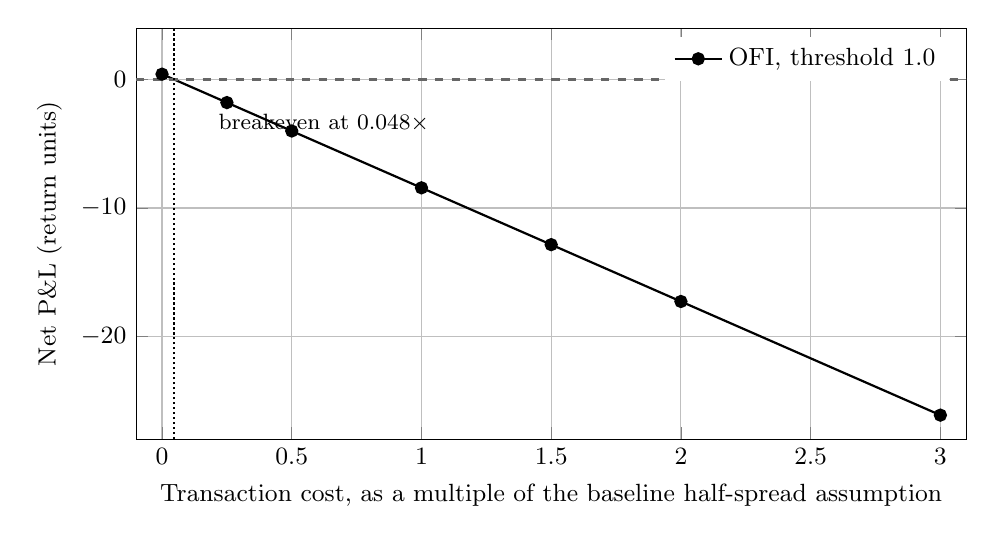
\begin{tikzpicture}
\begin{axis}[
  height=6.8cm,
  xlabel={Transaction cost, as a multiple of the baseline half-spread assumption},
  ylabel={Net P\&L (return units)},
  xmin=-0.1, xmax=3.1,
  ymin=-28, ymax=4,
  legend style={at={(0.98,0.98)},anchor=north east,draw=none},
]
\addplot[mark=*,thick] coordinates {(0,0.4217)(0.25,-1.7912)(0.5,-4.0040)(1.0,-8.4296)(1.5,-12.8552)(2.0,-17.2809)(3.0,-26.1322)};
\addlegendentry{OFI, threshold 1.0}
\addplot[black!60, thick, dashed, domain=-0.1:3.1, samples=2, forget plot] {0};
\draw[thick, densely dotted] (axis cs:0.0476,-28) -- (axis cs:0.0476,4);
\node[font=\footnotesize, anchor=west, align=left] at (axis cs:0.18,-3.4)
  {breakeven at $0.048\times$};
\end{axis}
\end{tikzpicture}
\caption{Where the strategy stops being profitable. Net P\&L crosses zero at 4.8\% of the assumed half-spread, so a twenty-fold error in the cost model would be needed to change the sign of the conclusion.}
\label{fig:costs}
\end{figure}

Figure~\ref{fig:costs} plots the sweep. \textbf{The breakeven cost multiple for OFI is 0.048.} The strategy is profitable only if crossing the spread costs less than 4.8\% of the half-spread. For the other signals it is lower still: 0.039 for queue imbalance and 0.040 for micro-price deviation.

That number is the paper's central economic result, and it is not close. A twenty-fold error in the cost model would be required to change the sign of the conclusion. No plausible refinement, and no realistic rebate, commission, or fee structure, moves a strategy that needs to pay 4.8\% of a half-spread into profitability.

\begin{table}[H]
\centering
\caption{Execution ladder, OFI at threshold 1.0.}
\label{tab:execution}
\begin{tabular}{rlrr}
\toprule
Level & Description & Gross P\&L & Net P\&L \\
\midrule
1 & Fill at mid, no cost        & 0.422 & $\mathbf{+0.422}$ \\
2 & Cross the spread            & 0.422 & $-8.430$ \\
3 & Half-spread plus slippage   & 0.422 & $-12.855$ \\
4 & Partial fills               & 0.397 & $-6.780$ \\
\bottomrule
\end{tabular}
\end{table}

Table~\ref{tab:execution} isolates why. The entire apparent edge lives in the execution assumption. Level~1 is the only profitable rung, and it assumes fills at the mid-price at zero cost.

\begin{remark}[On annualised Sharpe ratios]
A backtest reporting only level~1 would show a gross Sharpe of 0.032 per event, which annualises to 7{,}757. Scaling a Sharpe measured at 98-microsecond median event spacing by the square root of time assumes independence across events, which is the assumption the block bootstrap is there to test. Per-event Sharpe is the primary figure throughout.
\end{remark}

% =========================================================
\section{Adverse selection}
\label{sec:adverse}

If a strategy is profitable, it matters greatly whether the profit comes from providing liquidity and earning the spread, or from being picked off more slowly than average. The diagnostic, reported in Table~\ref{tab:adverse}, is the signed mid drift after a fill:
\begin{equation}
AS(h) = \operatorname{sign}(\text{trade}) \cdot \frac{m_{t+h} - m_t}{m_t}.
\label{eq:adverse}
\end{equation}

\begin{table}[H]
\centering
\caption{Mean adverse selection after 41{,}250 fills, in basis points. Quintiles are of the spread at the moment of the fill.}
\label{tab:adverse}
\begin{tabular}{rrrr}
\toprule
Horizon & All fills & Narrowest quintile & Widest quintile \\
\midrule
1 event   & $+0.010$ & $+0.004$ & $+0.015$ \\
5 events  & $+0.030$ & $+0.020$ & $+0.070$ \\
10 events & $+0.050$ & $+0.030$ & $+0.070$ \\
25 events & $+0.070$ & $+0.050$ & $+0.120$ \\
\bottomrule
\end{tabular}
\end{table}

Adverse selection is positive throughout, meaning the mid moves \emph{in favour} of the fill. The strategy is not being picked off. It is correctly anticipating direction, and the anticipation grows with horizon exactly as Section~\ref{sec:predictive} predicts.

The spread conditioning shows no clean monotone pattern, and the ordering reverses with horizon: the widest quintile leads at 5 events and trails badly at 25. I do not have an explanation I trust for that reversal and will not manufacture one.

\begin{remark}[A conditioning variable that was secretly an instrument label]
\label{rem:conditioning}
An earlier version of this table ranked the spread across the pooled panel rather than within each name, and reported a clean result: post-fill drift rose monotonically with spread, which read as ``the information is where the spread is wide''. It was an artefact. Median absolute spreads run from \$0.01 on INTC and MSFT to \$0.29 on GOOG, so a pooled quintile of absolute spread sorts tickers, not market states: the widest quintile was 99.9\% AAPL, AMZN, and GOOG, and the narrowest 99.1\% INTC and MSFT. The apparent spread effect was Table~\ref{tab:byinstrument} in disguised units. Ranking within instrument removes both the disguise and the pattern.
\end{remark}

At 25 events the fill is followed by 0.068 basis points of favourable drift, against median relative spreads of 2.6 to 5.9 basis points across the five names: one to three per cent of the entry cost.

% =========================================================
\section{Robustness}
\label{sec:robustness}

This section is structured as an attempt to destroy the result rather than a defence of it. Since the headline result is a negative one, the destruction runs in both directions: the loss must be robust, and the underlying prediction must be real.

\subsection{Is the prediction real?}
\label{sec:isreal}

\paragraph{Block-shifted randomisation.} The signal is circularly shifted in blocks, preserving its own autocorrelation while destroying its alignment with future returns, and the strategy is re-run 24 times per signal. Judged on \emph{gross} Sharpe, OFI, queue imbalance, and micro-price deviation all beat every shifted draw ($p = 0.04$, at the resolution floor). Spread does not ($p = 0.08$).

\begin{remark}[A trap I walked into]
\label{rem:nulltrap}
My first implementation judged this test on \emph{net} Sharpe. Under that version, spread also ``beat its own null'' despite negative gross P\&L. The reason is that shifting a signal changes \emph{when} it trades, and therefore what it pays: a strategy can beat a shifted null purely by trading at moments when the spread happens to be narrow. The net-based test was measuring turnover timing, not prediction. Gross isolates the only thing the shift is supposed to destroy. The synthetic controls never caught this, because their spread process has no intraday structure for the timing to exploit.
\end{remark}

\paragraph{Quantile response.} Bucketing OFI into deciles and measuring mean forward return at $h=10$ gives a cleanly monotone relationship across all ten buckets, from $-0.202$ basis points in the bottom decile to $+0.159$ in the top. Queue imbalance is monotone over the same range ($-0.277$ to $+0.233$), as is micro-price deviation ($-0.258$ to $+0.190$). Spread is flat and slightly negative throughout.

\subsection{Is the loss robust?}
\label{sec:isrobust}

\begin{table}[H]
\centering
\caption{Intraday period stability, OFI at threshold 1.0.}
\label{tab:periods}
\begin{tabular}{rlrrrr}
\toprule
Period & Window & Events & Gross P\&L & Net P\&L & Sharpe (net) \\
\midrule
1 & 09:30--10:48 & 244{,}942 & $+0.129$ & $-2.53$ & $-0.177$ \\
2 & 10:48--12:06 & 174{,}743 & $+0.067$ & $-1.40$ & $-0.175$ \\
3 & 12:06--13:24 & 157{,}368 & $+0.067$ & $-1.38$ & $-0.182$ \\
4 & 13:24--14:42 & 125{,}155 & $+0.059$ & $-1.16$ & $-0.190$ \\
5 & 14:42--16:00 & 251{,}621 & $+0.088$ & $-1.75$ & $-0.165$ \\
\bottomrule
\end{tabular}
\end{table}

In Table~\ref{tab:periods}, gross P\&L is positive in all five intraday periods and net P\&L is negative in all five, with net Sharpe confined to the range $-0.165$ to $-0.190$. The result is not an artefact of the open or the close.

\paragraph{Instrument stability.} Net P\&L is negative on all five instruments, from $-0.74$ on AAPL to $-2.95$ on MSFT, with net Sharpe between $-0.168$ and $-0.248$. No name is carrying or rescuing the result.

\paragraph{Threshold sensitivity.} Net P\&L improves monotonically as the threshold rises, from $-23.14$ at a threshold of 0.25 to $-0.96$ at 3.0. The strategy approaches breakeven only by approaching not trading at all: at a threshold of 3.0 it holds a position 1.4\% of the time and executes 3{,}581 trades instead of 100{,}891. Trading less is not a strategy; it is the absence of one.

\paragraph{Subsampling.} Net Sharpe worsens from $-0.177$ to $-0.306$ as the sampling stride goes from every event to every fifth, so the conclusion does not depend on snapshot frequency.

\paragraph{Walk-forward.} Five expanding folds within each instrument, with a purge gap, selecting signal and threshold on validation and evaluating once on test. Every fold's test block spans all five names. Zero folds have a positive test Sharpe. Mean test Sharpe is $-0.018$ against mean train Sharpe $-0.014$: the in-sample figure overstates the out-of-sample one by 0.004 Sharpe points per event.

\begin{remark}[The selection procedure prefers the non-signal]
\label{rem:selection}
The specification chosen on validation is spread at a threshold of 3.0 in four of the five folds, and micro-price deviation in the fifth. OFI, the signal with the strongest evidence in Section~\ref{sec:predictive} by a factor of two, is never selected. This is not a contradiction: selection here maximises validation Sharpe, every candidate loses money, and the least-bad way to lose money is to trade as little as possible. Spread at a high threshold trades least. A selection criterion that rewards minimal trading when nothing is profitable will reliably choose the weakest signal, and reporting the winner of that contest as though it were a finding would be an error the walk-forward machinery does nothing to prevent.
\end{remark}

\paragraph{Selection inflation.} Across 24 candidate specifications, the in-sample winner scores $-0.016$ in sample and $-0.004$ out of sample, which is also the best available out-of-sample score, so measured inflation is negative and regret against an oracle is zero. This is not evidence of a well-behaved selection procedure. It is what happens when every candidate loses money: picking the least-bad in sample happens to pick the least-bad out of sample, and the diagnostic has nothing to detect. On a dataset with genuine winners it would.

\paragraph{Confidence.} Block bootstrap on net P\&L gives a Sharpe of $-0.177$ with a 95\% interval of $[-0.182, -0.174]$, excluding zero. The Newey--West $t$-statistic \cite{NeweyWest1987} is $-105.9$. The loss is not a sampling accident.

% =========================================================
\section{Failure analysis}
\label{sec:failure}

Each signal fails at a specific gate, and the gate differs in each case.

\paragraph{Spread fails at gate one.} Its cross-sectional $t$-statistic is 1.07 and its sign does not hold across instruments, being positive on the three wide-spread names and negative on the two penny-spread ones. It also fails the shifted-null test on gross Sharpe. There is no directional information in the spread at the top of the book on this panel.

\paragraph{Micro-price deviation fails at gate two, in a specific sense.} It passes cross-sectional significance comfortably, but Section~\ref{sec:redundancy} shows it is the same signal as queue imbalance, with an incremental out-of-sample $R^2$ of $-0.0006$. It does not fail on its own terms. It fails to be a fourth signal.

\paragraph{Queue imbalance and OFI fail at gate four.} Both are genuinely predictive on all five instruments, both survive correction across 1{,}080 hypotheses, both beat their shifted nulls on gross Sharpe, and both generate positive gross P\&L. Both lose money by a factor of roughly twenty after costs.

The single assumption carrying the entire result is the execution assumption. At level~1, mid-price fills at zero cost, OFI earns a gross Sharpe of 0.032 per event. At level~2, crossing the spread, it loses 0.177. Nothing else in the analysis is anywhere near as decisive: not the threshold, not the horizon, not the choice of signal, not the regime conditioning.

\textbf{The number to remember: a strategy trading OFI at the top of the book must execute at 4.8\% of the half-spread to break even.} That is not a cost model awaiting refinement. It is a statement that the information exists at a scale roughly twenty times smaller than the price of acting on it.

\begin{remark}[What this does not prove]
\label{rem:notprove}
It does not prove that limit order book information is untradable. It proves that it is untradable \emph{by crossing the spread on every signal}. A liquidity-providing strategy earning the spread rather than paying it faces different arithmetic, and Section~\ref{sec:adverse} supplies its key input: resting orders filled by this signal are followed by favourable drift. That extension requires the queue-position modelling this framework declares and does not implement.
\end{remark}

% =========================================================
\section{Conclusion}
\label{sec:conclusion}

\begin{table}[H]
\centering
\caption{Final verdict. Four gates, four signals.}
\label{tab:verdict}
\begin{tabular}{lllll>{\bfseries}l}
\toprule
Signal & Predictive & Correction & Net profitable & Beats null & All gates \\
\midrule
OFI                   & yes ($t=18.0$) & yes & \textbf{no} ($0.048\times$) & yes & no \\
Queue imbalance       & yes ($t=7.3$)  & yes & \textbf{no} ($0.039\times$) & yes & no \\
Micro-price deviation & yes ($t=7.6$)  & yes & \textbf{no} ($0.040\times$) & yes & no \\
Spread                & no ($t=1.1$)   & no  & no & no & no \\
\bottomrule
\end{tabular}
\end{table}

Nothing in Table~\ref{tab:verdict} survives all four gates.

Three findings are worth separating from that headline.

\paragraph{Information is abundant and cheap to measure.} Three of four signals predict short-horizon returns with rank ICs between 0.10 and 0.19, holding the same sign on every instrument, surviving correction across 1{,}080 hypotheses, and producing monotone decile responses. The prediction is real and easy to find.

\paragraph{Which signal works depends on the book.} OFI dominates on wide-spread, thin-queue names; queue imbalance dominates on penny-spread, deep-queue names; the ordering flips completely between the two groups, and the same pattern reappears within instruments when conditioning on depth. A study on a single instrument would report one of these and call it the answer.

\paragraph{None of it survives the spread.} The best signal breaks even at 4.8\% of the assumed half-spread. Costs consume 2{,}099\% of gross profit at the baseline assumption, and the entire apparent edge lives in the one execution rung that assumes free fills at the mid.

The methodological claim generalises past this dataset. Correlation, cross-sectionally general prediction, gross profit, and net profit are four separate claims, and the distance between the third and the fourth is where most limit order book research quietly ends. Reporting the first three and stopping is not a small omission. On this panel it is the difference between an annualised Sharpe in the thousands and a loss of twenty times gross.

The framework was built to make that failure visible rather than avoidable. It did, twice: once for the signals, and once for two of my own measurement choices, in Remarks~\ref{rem:pooling} and~\ref{rem:nulltrap}.

% =========================================================
\appendix
\newpage

\section{Appendix A: Machinery validation on synthetic controls}
\label{sec:controls}

A null result is only meaningful if the machinery could have found a positive one. Three synthetic markets establish that.

\subsection{Null control}
No relationship between book state and future returns by construction. Peak absolute rank IC across all four signals is below 0.014, no signal is flagged predictive, and no economic gate is cleared.

\subsection{Planted OFI control}
A known OFI relationship, uniformly active. OFI is recovered at a rank IC of 0.280, clears multiple-testing correction, and beats its shifted null. It is still not net profitable, with a breakeven cost multiple of 0.27. The gap between statistical and economic significance reproduces on data where the statistical part is known to be real.

\subsection{Regime control}
The relationship is active only in a persistent wide-spread state. Pooled rank IC understates it at 0.19, and conditioning on the \emph{inferred} spread regime recovers the structure: 0.083 in tight spreads, 0.216 in medium, 0.270 in wide. The simulator's true regime label is never exposed to the pipeline.

\subsection{Calibration}
Across independent null realisations, mean rank IC is $-0.006$ with a standard deviation of 0.021, and the block-permutation test rejects at most twice in five.

\begin{remark}[What controls cannot establish]
Remark~\ref{rem:nulltrap} records a bug the synthetic controls did not catch, because the simulated spread has no intraday structure for a shifted signal to exploit. Controls establish that the machinery works on the phenomena they model. They cannot establish that it works on phenomena they omit, which is an argument for running on real data early rather than perfecting the simulator.
\end{remark}

% =========================================================
\section{Appendix B: Parameters}
\label{sec:params}

Every number in this paper depends on choices that a single command reproduces but that the prose alone does not pin down. Table~\ref{tab:params} lists them. The decisive one is the first row: order flow imbalance normalised by trailing depth has a pooled rank IC at $h=1$ of 0.083, and unnormalised it has 0.037. A reader who reimplemented the signal from Section~\ref{sec:ofi} without the normalisation would fail to reproduce Table~\ref{tab:pooled} and would have no way of knowing why.

\begin{table}[H]
\centering
\caption{Parameters that change published numbers.}
\label{tab:params}
\begin{tabular}{llp{6.4cm}}
\toprule
Parameter & Value & What it sets \\
\midrule
\texttt{ofi.window}                & 20     & Events in the OFI rolling sum \\
\texttt{ofi.depth\_window}         & 200    & Trailing window for the depth normaliser. Decisive: unnormalised, OFI's $h{=}1$ IC falls from 0.083 to 0.037 \\
\texttt{zscore\_window}            & 10{,}000 & Trailing window for signal standardisation; sets exposure, turnover, and every P\&L figure \\
\texttt{threshold}                 & 1.0    & Entry threshold in trailing standard deviations \\
\texttt{block}                     & 2{,}000 & Bootstrap block length and minimum admissible circular shift \\
\texttt{n\_boot}                   & 150    & Bootstrap draws behind every interval \\
\texttt{n\_perm}                   & exact  & The shift test enumerates all $\approx 950{,}000$ shifts \\
\texttt{regime\_window}            & 10{,}000 & Trailing window for regime terciles, Table~\ref{tab:regimes} \\
\texttt{vol\_window}               & 500    & Realised volatility window, Table~\ref{tab:regimes}'s volatility row \\
\texttt{max\_relative\_jump}       & 0.05   & Cleaning rule 8 \\
\texttt{purge}                     & 101    & Walk-forward purge gap, one more than the longest horizon \\
\texttt{min\_train\_fraction}      & 0.4    & Walk-forward fold geometry \\
\texttt{slippage\_fraction\_of\_spread} & 0.25 & Execution level 3 \\
\texttt{fill\_ratio}               & 0.6    & Execution level 4 \\
\texttt{randomisation\_draws}      & 24     & Shifted-null draws per signal, floor $p = 0.04$ \\
\bottomrule
\end{tabular}
\end{table}

% =========================================================
\section{Appendix C: Known limitations}
\label{sec:limitations}

\begin{enumerate}
\item \textbf{One trading session.} All five instruments cover the same day. The session machinery is exercised and tested, but nothing here speaks to day-to-day persistence, and period stability degrades to intraday sub-periods. This is the largest limitation and the one I would fix first.

\item \textbf{Level 1 only.} The export has ten levels. OFI is computed at the touch, which is defensible and standard, but a level-2 to level-5 variant is untested and might behave differently on the deep-queue names where the touch is least informative.

\item \textbf{The circular-shift permutation null is mildly anti-conservative.} On the synthetic null control its distribution is roughly 40\% narrower than the spread of rank IC across independent realisations, because shifting preserves each series' own autocorrelation but not the variation between realised paths. Single-sample $p$-values should be read as optimistic.

\item \textbf{The gate-level randomisation null is still sampled}, at 24 draws per signal, so its $p$-values floor at 0.04. Only the IC table uses the exact enumeration. A signal cannot clear that gate more convincingly than 0.04 however strong it is.

\item \textbf{The circular-shift null assumes one realisation is informative about the ensemble.} It preserves each series' own autocorrelation but not the variation between independent realised paths, and on the synthetic control its distribution is roughly 40\% narrower than the across-seed spread of rank IC. Exactness removes the sampling error, not this bias.

\item \textbf{Rank IC bootstraps resample pre-computed ranks}, which are not recomputed within each draw. A deliberate approximation that makes several hundred permutations affordable on a million-row panel.

\item \textbf{Horizons stop too early.} No signal decays to half its peak within 100 events. The range should have extended to 250 or 500.

\item \textbf{Queue-aware passive execution is not implemented.} Execution level~5 raises rather than approximates, so no result here depends on a fill model that was never written. Given Section~\ref{sec:failure}, it is also the most important missing piece.

\item \textbf{The selection criterion rewards inactivity.} Remark~\ref{rem:selection}: because no candidate is profitable, validation Sharpe is maximised by whichever specification trades least, and the procedure selects the paper's declared non-signal in four folds of five. A walk-forward apparatus does not protect against a criterion that is pointing the wrong way.

\item \textbf{Taking, not making.} Every strategy tested crosses the spread. The conclusion concerns liquidity-taking strategies at the top of the book, and does not transfer to market making.
\end{enumerate}

% =========================================================
\section{Appendix D: Reproducibility}
\label{sec:repro}

Every table in this paper is produced by:

\begin{lstlisting}[style=py, caption={Reproducing the full result set.}]
python run_experiment.py configs/lobster_panel.yaml
python experiments/finish_gates.py configs/lobster_panel.yaml
\end{lstlisting}

The full run takes about five minutes on 953{,}829 events, split into two commands because the per-signal gate stage is over a hundred backtests on its own. Each config carries a content hash, recorded in the run summary. Raw data is read-only, cleaning writes to a separate directory, and the audit trail is Table~\ref{tab:cleaning}.

The repository ships 80 tests covering order book invariants, every branch of the OFI definition against hand-constructed books, session-boundary leakage, cost and backtest accounting identities, split geometry, and recovery of planted relationships from synthetic data. Notebooks are used for exploration only. Once an experiment is intended for reporting it moves into the pipeline, which is what prevents a reported result from being quietly re-tuned.

The LOBSTER samples are free academic downloads from \url{https://lobsterdata.com/info/DataSamples.php} and are not redistributed with the code. The repository is at \url{https://github.com/study-holic/q1-lob-alpha}; the release tagged \texttt{v1.0-paper} is the state from which every number in this paper was produced.

% =========================================================
\newpage
\begin{thebibliography}{99}

\bibitem{Bailey2014}
D.\,H. Bailey and M. L\'opez de Prado,
``The Deflated Sharpe Ratio: Correcting for Selection Bias, Backtest Overfitting, and Non-Normality,''
\textit{Journal of Portfolio Management}, 40(5), 94--107, 2014.

\bibitem{Benjamini1995}
Y. Benjamini and Y. Hochberg,
``Controlling the False Discovery Rate: A Practical and Powerful Approach to Multiple Testing,''
\textit{Journal of the Royal Statistical Society~B}, 57(1), 289--300, 1995.

\bibitem{Cont2014}
R. Cont, A. Kukanov, and S. Stoikov,
``The Price Impact of Order Book Events,''
\textit{Journal of Financial Econometrics}, 12(1), 47--88, 2014.

\bibitem{Harvey2016}
C.\,R. Harvey, Y. Liu, and H. Zhu,
``$\ldots$ and the Cross-Section of Expected Returns,''
\textit{Review of Financial Studies}, 29(1), 5--68, 2016.

\bibitem{Huang2011}
R. Huang and T. Polak,
``LOBSTER: Limit Order Book Reconstruction System,''
SSRN Working Paper 1977207, 2011.

\bibitem{Kercheval2015}
A.\,N. Kercheval and Y. Zhang,
``Modelling High-Frequency Limit Order Book Dynamics with Support Vector Machines,''
\textit{Quantitative Finance}, 15(8), 1315--1329, 2015.

\bibitem{NeweyWest1987}
W.\,K. Newey and K.\,D. West,
``A Simple, Positive Semi-Definite, Heteroskedasticity and Autocorrelation Consistent Covariance Matrix,''
\textit{Econometrica}, 55(3), 703--708, 1987.

\bibitem{Stoikov2018}
S. Stoikov,
``The Micro-Price: A High-Frequency Estimator of Future Prices,''
\textit{Quantitative Finance}, 18(12), 1959--1966, 2018.

\end{thebibliography}

\end{document}
